\documentclass[a4paper,12pt]{article}

\usepackage[T2A]{fontenc}
\usepackage[utf8]{inputenc}
\usepackage[russian]{babel}
\usepackage{cmap}

\usepackage{amsmath,amssymb,mathtools}
\usepackage[a4paper,left=25mm,right=15mm,top=20mm,bottom=20mm]{geometry}
\usepackage{indentfirst}
\usepackage{graphicx}
\usepackage{float}
\usepackage{caption}
\usepackage{booktabs}
\usepackage{enumitem}
\usepackage{titlesec}
\usepackage[unicode,hidelinks]{hyperref}

\captionsetup{labelsep=endash,font=small,skip=4pt}
\addto\captionsrussian{\renewcommand{\figurename}{Рисунок}\renewcommand{\tablename}{Таблица}}

\titleformat{\section}{\normalfont\large\bfseries}{\thesection}{0.6em}{}
\titleformat{\subsection}{\normalfont\normalsize\bfseries}{\thesubsection}{0.6em}{}
\titlespacing*{\section}{0pt}{14pt}{6pt}
\titlespacing*{\subsection}{0pt}{10pt}{4pt}

\setlength{\parindent}{1.25cm}
\setlength{\emergencystretch}{1.5em}
\linespread{1.1}
\setlist{itemsep=1pt,topsep=3pt}

\graphicspath{{figures/}}
\newcommand{\code}[1]{\texttt{#1}}

\begin{document}

\begin{center}
  {\Large\bfseries Одномерное волновое уравнение:\\[2pt]
   метод характеристик и функция Грина\par}
  \vspace{6pt}
  {Отчёт по заданиям А и Б\par}
  \vspace{4pt}
  {Выполнили: \rule{8cm}{0.4pt}\par}
\end{center}

\noindent\textbf{А.} Функция, которая строит решение волнового уравнения на
полупрямой методом характеристик и выдаёт график решения для момента времени~$t$.

\noindent\textbf{Б.} Функция, которая строит решение задачи Коши на прямой через
функцию Грина и выдаёт анимированные графики решения и функции Грина на отрезке
времени длительностью~$T$.

Язык~--- Python. Все вычисления выполняют функции, написанные самостоятельно:
построение сетки, формулы трапеций и Симпсона, линейная интерполяция по таблице
(\code{wavelab/numint.py}), функция Грина и сборка решения. Библиотеки
\code{numpy} и \code{scipy} не используются. Из стандартной библиотеки взят
только модуль \code{math} (элементарные функции $\sin$, $\cos$, $\exp$),
\code{matplotlib} и \code{tkinter}~--- только для рисования и окна программы.

% ======================================================================
\section{Задание А. Полупрямая, метод характеристик}

\subsection{Постановка задачи}

\begin{equation}\label{eq:A}
\begin{gathered}
  u_{tt}=a^{2}u_{xx},\qquad x>0,\ t>0,\\
  u(x,0)=\varphi(x),\qquad u_t(x,0)=\psi(x),\qquad x\ge 0,
\end{gathered}
\end{equation}
и одно из граничных условий при $x=0$, $t\ge 0$:
\begin{align*}
  \text{I рода:}\quad   & u(0,t)=\mu(t);\\
  \text{II рода:}\quad  & u_x(0,t)=\nu(t);\\
  \text{III рода:}\quad & u_x(0,t)-h\,u(0,t)=\omega(t).
\end{align*}
\textbf{Вариант группы}~--- условие I рода, правая часть которого задана суммой
двух функций:
\begin{equation}\label{eq:variant}
  u(0,t)=\mu(t)+g(t),\qquad t\ge 0 .
\end{equation}
Функции $\varphi$, $\psi$, $\mu$, $g$ и числа $a$, $t$ вводит пользователь.
Условия II и III рода реализованы дополнительно (род условия~--- параметр).

\subsection{Метод}

Характеристики уравнения~--- прямые $x-at=C$ и $x+at=C$. В переменных
$\xi=x-at$, $\eta=x+at$ уравнение принимает вид $u_{\xi\eta}=0$, поэтому
\begin{equation}\label{eq:FG}
  u(x,t)=F(x-at)+G(x+at).
\end{equation}

\textbf{Шаг 1: начальные условия.} При $z\ge 0$ из $F(z)+G(z)=\varphi(z)$,
$-aF'(z)+aG'(z)=\psi(z)$ получаем
\begin{equation}\label{eq:FGinit}
  G(z)=\frac{\varphi(z)}{2}+\frac{\Psi(z)}{2a},\qquad
  F(z)=\frac{\varphi(z)}{2}-\frac{\Psi(z)}{2a},\qquad
  \Psi(z)=\int_{0}^{z}\psi(s)\,ds .
\end{equation}
Аргумент $x+at$ всегда неотрицателен, поэтому $G$ известна полностью.
Если $x\ge at$, то и $F$ известна, и~\eqref{eq:FG} даёт формулу Даламбера:
до точки $x$ влияние границы ещё не дошло.

\textbf{Шаг 2: граничное условие.} Если $x<at$, характеристика $x-at=-y$
($y=at-x>0$) выходит не с оси $t=0$, а с границы $x=0$ в момент $t_0=y/a$.
Значение $F(-y)$ находим, подставив~\eqref{eq:FG} в граничное условие.
\begin{itemize}
  \item I рода: $F(-at)+G(at)=\mu(t)$, откуда
        \begin{equation}\label{eq:F1}
          F(-y)=\mu\!\left(\frac{y}{a}\right)-G(y).
        \end{equation}
  \item III рода: $F'(-at)+G'(at)-h\bigl[F(-at)+G(at)\bigr]=\omega(t)$.
        Это линейное ОДУ первого порядка для $F$; его решение с условием
        $F(0)=G(0)=\varphi(0)/2$:
        \begin{equation}\label{eq:F3}
          F(-y)=G(y)-W(y),\qquad
          W(y)=e^{-hy}\int_{0}^{y}e^{hq}\Bigl[2h\,G(q)+\omega\!\left(\frac{q}{a}\right)\Bigr]dq .
        \end{equation}
  \item II рода~--- частный случай $h=0$:
        $W(y)=\displaystyle\int_{0}^{y}\nu\!\left(\frac{q}{a}\right)dq
        =a\int_{0}^{y/a}\nu(p)\,dp$.
\end{itemize}

\textbf{Итог} при $x<at$:
\begin{align*}
  \text{I рода:}\quad &
  u=\mu\!\left(t-\frac{x}{a}\right)+\frac{\varphi(x+at)-\varphi(at-x)}{2}
    +\frac{1}{2a}\int_{at-x}^{x+at}\psi(s)\,ds;\\
  \text{II рода:}\quad &
  u=\frac{\varphi(x+at)+\varphi(at-x)}{2}
    +\frac{1}{2a}\Bigl[\int_{0}^{at-x}\!\!\psi\,ds+\int_{0}^{x+at}\!\!\psi\,ds\Bigr]
    -a\int_{0}^{t-x/a}\nu(p)\,dp;\\
  \text{III рода:}\quad &
  u=G(at-x)+G(x+at)-W(at-x).
\end{align*}
Для варианта~\eqref{eq:variant} в формуле I рода вместо $\mu$ стоит $\mu+g$:
\begin{equation}\label{eq:answer}
  u(x,t)=
  \begin{cases}
    \dfrac{\varphi(x-at)+\varphi(x+at)}{2}
      +\dfrac{1}{2a}\displaystyle\int_{x-at}^{x+at}\psi(s)\,ds, & x\ge at,\\[10pt]
    \mu\!\left(t-\dfrac{x}{a}\right)+g\!\left(t-\dfrac{x}{a}\right)
      +\dfrac{\varphi(x+at)-\varphi(at-x)}{2}
      +\dfrac{1}{2a}\displaystyle\int_{at-x}^{x+at}\psi(s)\,ds, & x<at.
  \end{cases}
\end{equation}
Задача линейна, поэтому это сумма решений трёх задач: с начальными данными
и закреплённым концом, с граничным режимом $\mu$ и с граничным режимом $g$.

При $\varphi=\psi=0$ формулы переходят в формулы лекции~3:
$u=\mu(t-x/a)$, $u=-a\int_{0}^{t-x/a}\nu(p)\,dp$ и
$u=-a\,e^{h(x-at)}\int_{0}^{t-x/a}\omega(s)e^{has}\,ds$.

\subsection{Реализация}

Функция из файла \code{wavelab/halfline.py}
\begin{center}
  \code{solve\_halfline(x, t, a, phi, psi, kind, g, h)}
\end{center}
работает так:
\begin{enumerate}
  \item строит сетку $z_k$ на отрезке $[0,\ \max x+at]$ и считает $\Psi(z_k)$
        формулой трапеций с накоплением (функция \code{cumtrapz});
        значения между узлами берутся линейной интерполяцией (функция \code{interp});
  \item для условий II и III рода считает $W(z_k)$ по рекуррентной формуле
        (трапеции с точным множителем $q=e^{-h\Delta z}$):
        $W_{k+1}=q\bigl(W_k+\tfrac{\Delta z}{2}r_k\bigr)+\tfrac{\Delta z}{2}r_{k+1}$,
        где $r=2hG+\omega(z/a)$;
  \item в каждой точке $x$ выбирает $F$ по~\eqref{eq:FGinit}, если $x\ge at$,
        и по~\eqref{eq:F1} или~\eqref{eq:F3}, если $x<at$, и складывает с $G(x+at)$.
\end{enumerate}
Таблицы $\Psi$ и $W$ хранит класс \code{HalfLine}: они строятся один раз,
после чего решение быстро вычисляется для любого момента времени (так работает ползунок в приложении).

Программа \code{task\_a.py} запрашивает данные у пользователя, вызывает эту
функцию с граничной функцией $\mu(t)+g(t)$ и рисует график: решение в момент $t$,
начальный профиль и характеристику $x=at$ (рисунок~\ref{fig:a-run}). Правее
характеристики решение даёт формула Даламбера (полуволна, ушедшая вправо),
левее~--- граничный режим и отражённая полуволна.

\begin{figure}[H]
  \centering
  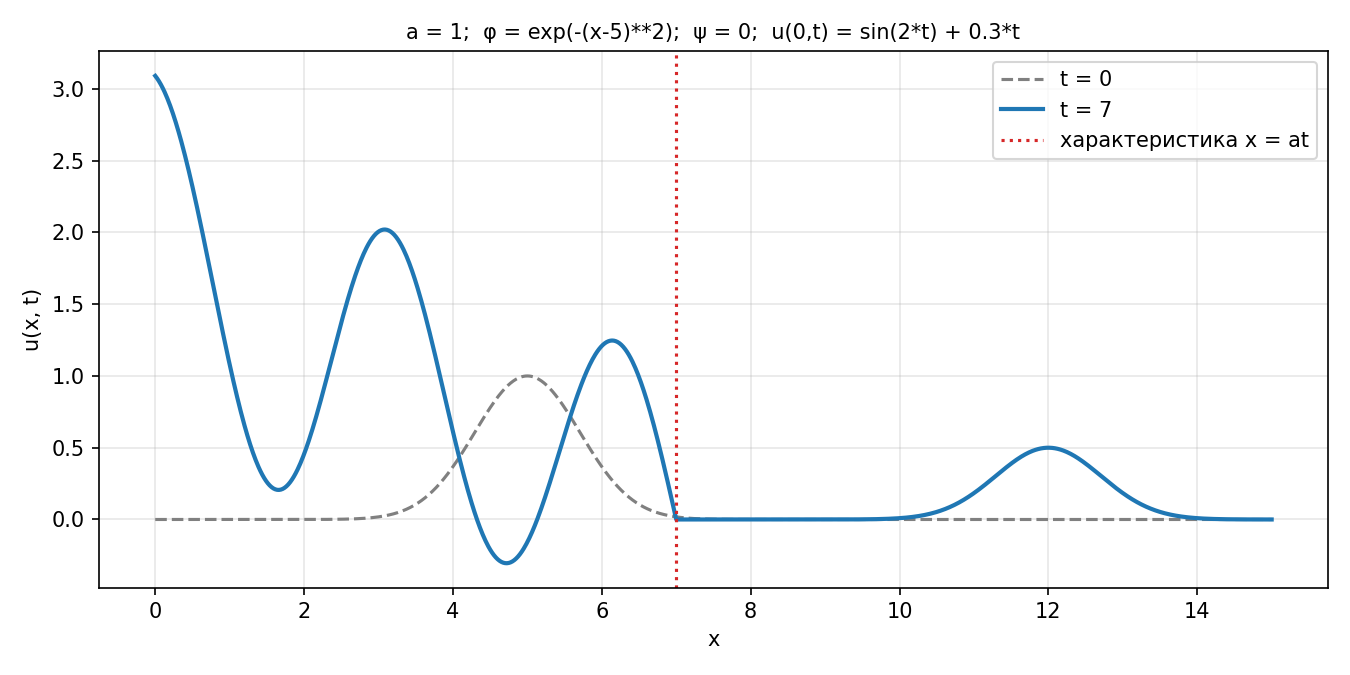
\includegraphics[width=0.85\textwidth]{a_run.png}
  \caption{Результат работы \code{task\_a.py}: $a=1$, $\varphi=e^{-(x-5)^2}$, $\psi=0$,
           $u(0,t)=\sin 2t+0{,}3t$, $t=7$}
  \label{fig:a-run}
\end{figure}

\subsection{Примеры}

На рисунке~\ref{fig:a-ex} $a=1$, $\psi=0$. Слева вверху~--- нулевые начальные
данные и граничный режим $u(0,t)=\sin 2t$: возмущение занимает область $x<at$.
В остальных примерах $\varphi=e^{-(x-5)^2}$: горб распадается на две полуволны,
левая отражается от границы. От закреплённого конца она возвращается
перевёрнутой, от свободного~--- без переворота, при условии III рода форма
отражённой волны искажается.

\begin{figure}[H]
  \centering
  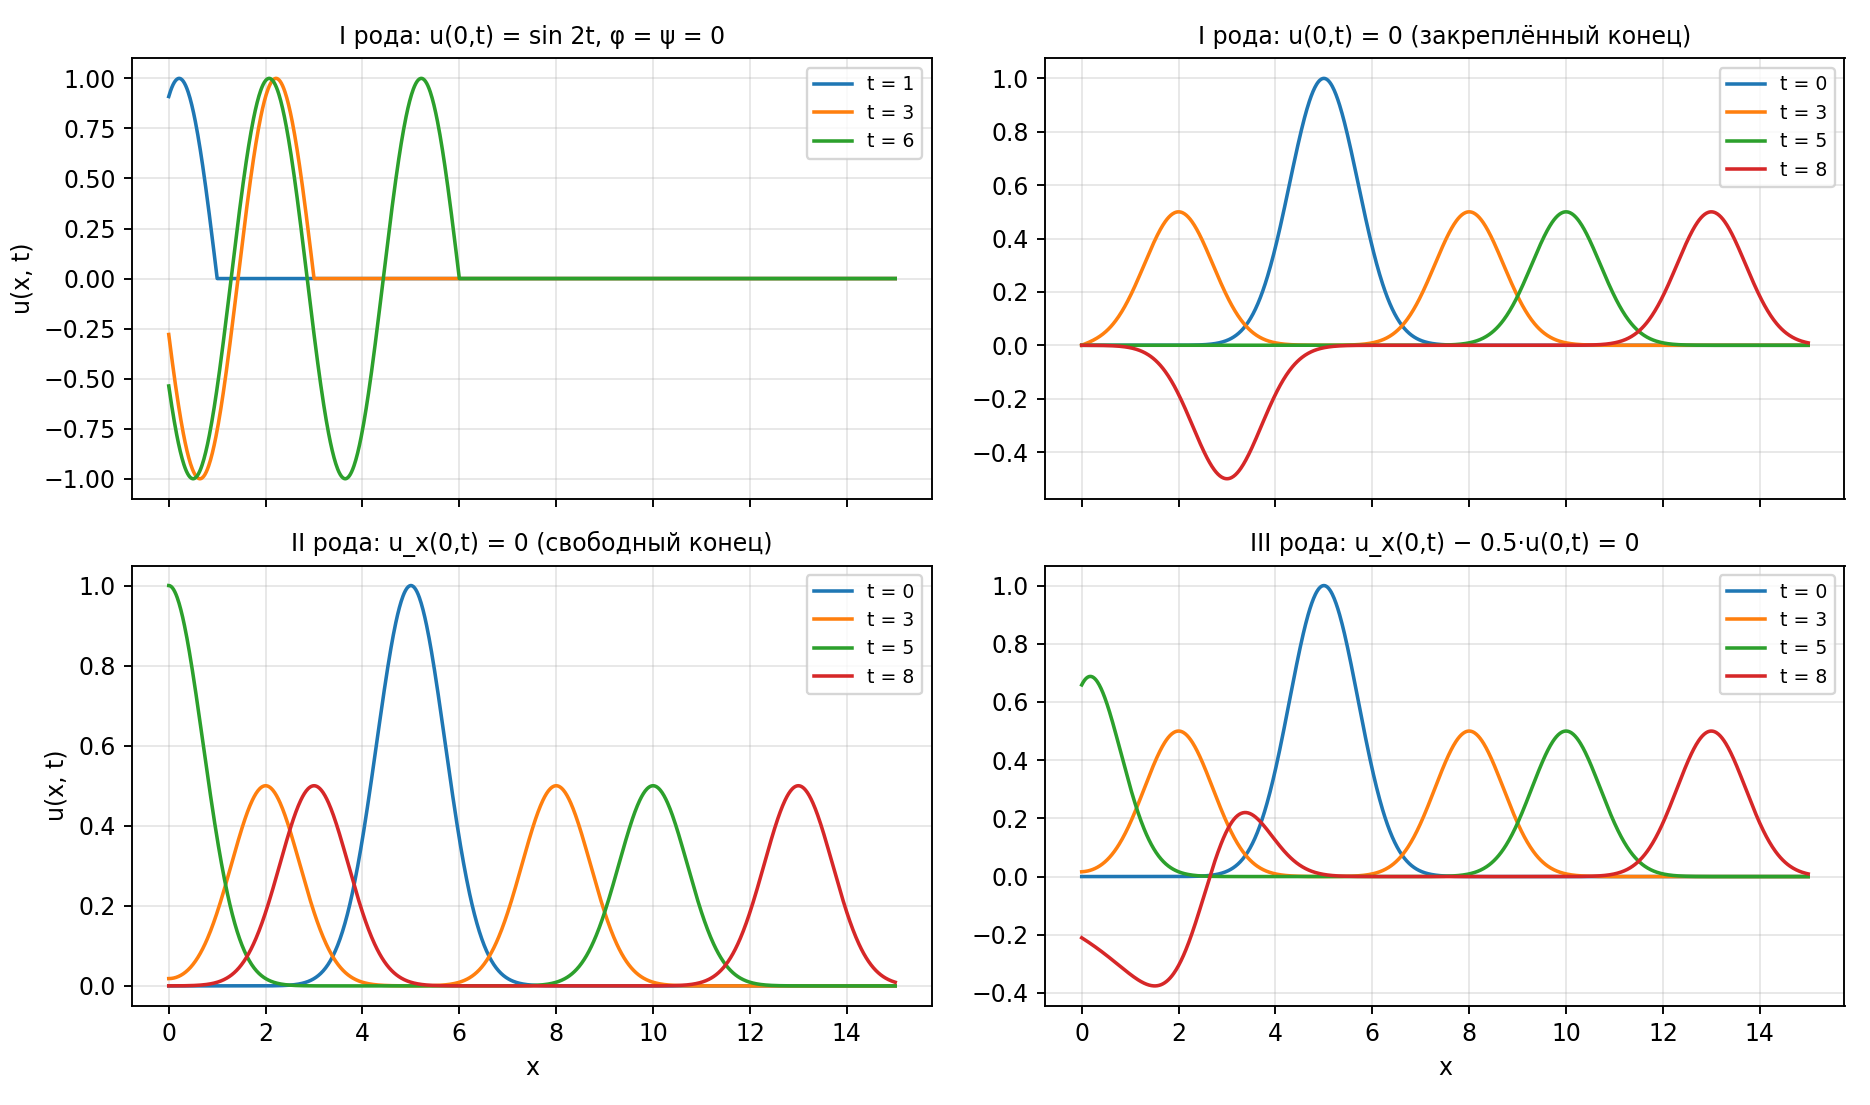
\includegraphics[width=\textwidth]{a_examples.png}
  \caption{Решение на полупрямой при трёх родах граничного условия}
  \label{fig:a-ex}
\end{figure}

\subsection{Проверка}

Взято точное решение $u=\sin(x-at)+\cos 2(x+at)$ при $a=2$, $h=0{,}7$; по нему
вычислены $\varphi$, $\psi$, $\mu$, $\nu$, $\omega$ и переданы программе.
Для всех трёх родов условия при $t=0;\ 0{,}5;\ 1{,}7;\ 4$ и $0\le x\le 12$
отклонение от точного решения меньше $10^{-5}$. Отдельно проверены формулы
лекции~3 для нулевых начальных данных, отражение горба от закреплённого
и свободного концов и принцип суперпозиции для варианта~\eqref{eq:variant} (файл \code{tests/test\_halfline.py}).

% ======================================================================
\section{Задание Б. Задача Коши на прямой, функция Грина}

\subsection{Постановка задачи и формулы}

\begin{equation}\label{eq:B}
\begin{gathered}
  u_{tt}=a^{2}u_{xx}+f(x,t),\qquad -\infty<x<\infty,\ t>0,\\
  u(x,0)=\varphi(x),\qquad u_t(x,0)=\psi(x).
\end{gathered}
\end{equation}
Функция Грина~--- отклик на единичный мгновенный импульс в точке $\xi$
в момент $t=0$ (лекция~4):
\begin{equation}\label{eq:G}
  G(x,\xi,t)=
  \begin{cases}
    \dfrac{1}{2a}, & |x-\xi|\le at,\\[6pt]
    0, & |x-\xi|>at.
  \end{cases}
\end{equation}
Решение задачи~\eqref{eq:B}:
\begin{equation}\label{eq:uG}
  u(x,t)=\int_{-\infty}^{\infty}\!G_t(x,\xi,t)\,\varphi(\xi)\,d\xi
        +\int_{-\infty}^{\infty}\!G(x,\xi,t)\,\psi(\xi)\,d\xi
        +\int_{0}^{t}\!\!\int_{-\infty}^{\infty}\!G(x,\xi,t-\tau)\,f(\xi,\tau)\,d\xi\,d\tau .
\end{equation}

\subsection{Реализация}

Функция \code{green(x, xi, t, a)} вычисляет~\eqref{eq:G}. Функция
\code{solve\_cauchy(x, t, a, phi, psi, f)} (файл \code{wavelab/green.py})
считает три слагаемых~\eqref{eq:uG}.
\begin{enumerate}
  \item Первое слагаемое. Функция $G$ ступенчатая, её производная по времени
        $G_t=\tfrac12\bigl[\delta(\xi-(x-at))+\delta(\xi-(x+at))\bigr]$, поэтому
        интеграл берётся точно:
        $\displaystyle\int G_t\,\varphi\,d\xi=\frac{\varphi(x-at)+\varphi(x+at)}{2}$.
  \item Второе слагаемое. Вне отрезка $[x-at,\ x+at]$ функция $G$ равна нулю,
        поэтому узлы берутся только на нём: $\xi_j=x+at\,s_j$, $s_j\in[-1,1]$;
        интеграл от $G\cdot\psi$ считается по формуле Симпсона (201 узел,
        функция \code{green\_integral}, в каждом узле вызывается \code{green}).
  \item Третье слагаемое. Внешний интеграл по $\tau\in[0,t]$~--- формула
        Симпсона (101 узел), внутренний~--- как во втором слагаемом,
        но с радиусом $a(t-\tau)$.
\end{enumerate}
Программа \code{task\_b.py} запрашивает $a$, $\varphi$, $\psi$, $f$, $T$, границы
графика и точку $\xi$, считает решение и функцию Грина на кадрах
$t_k\in[0,T]$ и показывает анимацию из двух графиков: сверху $u(x,t)$, снизу
$G(x,\xi,t)$. Анимация сохраняется в файл GIF. Для анимации число узлов
уменьшено (81 по $\xi$; при $f\ne 0$~--- 31 по $\xi$ и 31 по $\tau$), чтобы расчёт
121 кадра занимал секунды; погрешность при этом порядка $10^{-4}$--$10^{-3}$.

\subsection{Примеры}

Рисунок~\ref{fig:b-frames}~--- кадры анимации для примера лекции~3:
$\varphi=\max(1-|x|,0)$, $\psi=0$, $f=0$. Треугольник распадается на два
треугольника половинной высоты, бегущих в разные стороны со скоростью $a$.
Функция Грина~--- прямоугольник высотой $1/(2a)$ на отрезке
$[\xi-at,\ \xi+at]$, который расширяется со скоростью $a$ в обе стороны.

\begin{figure}[H]
  \centering
  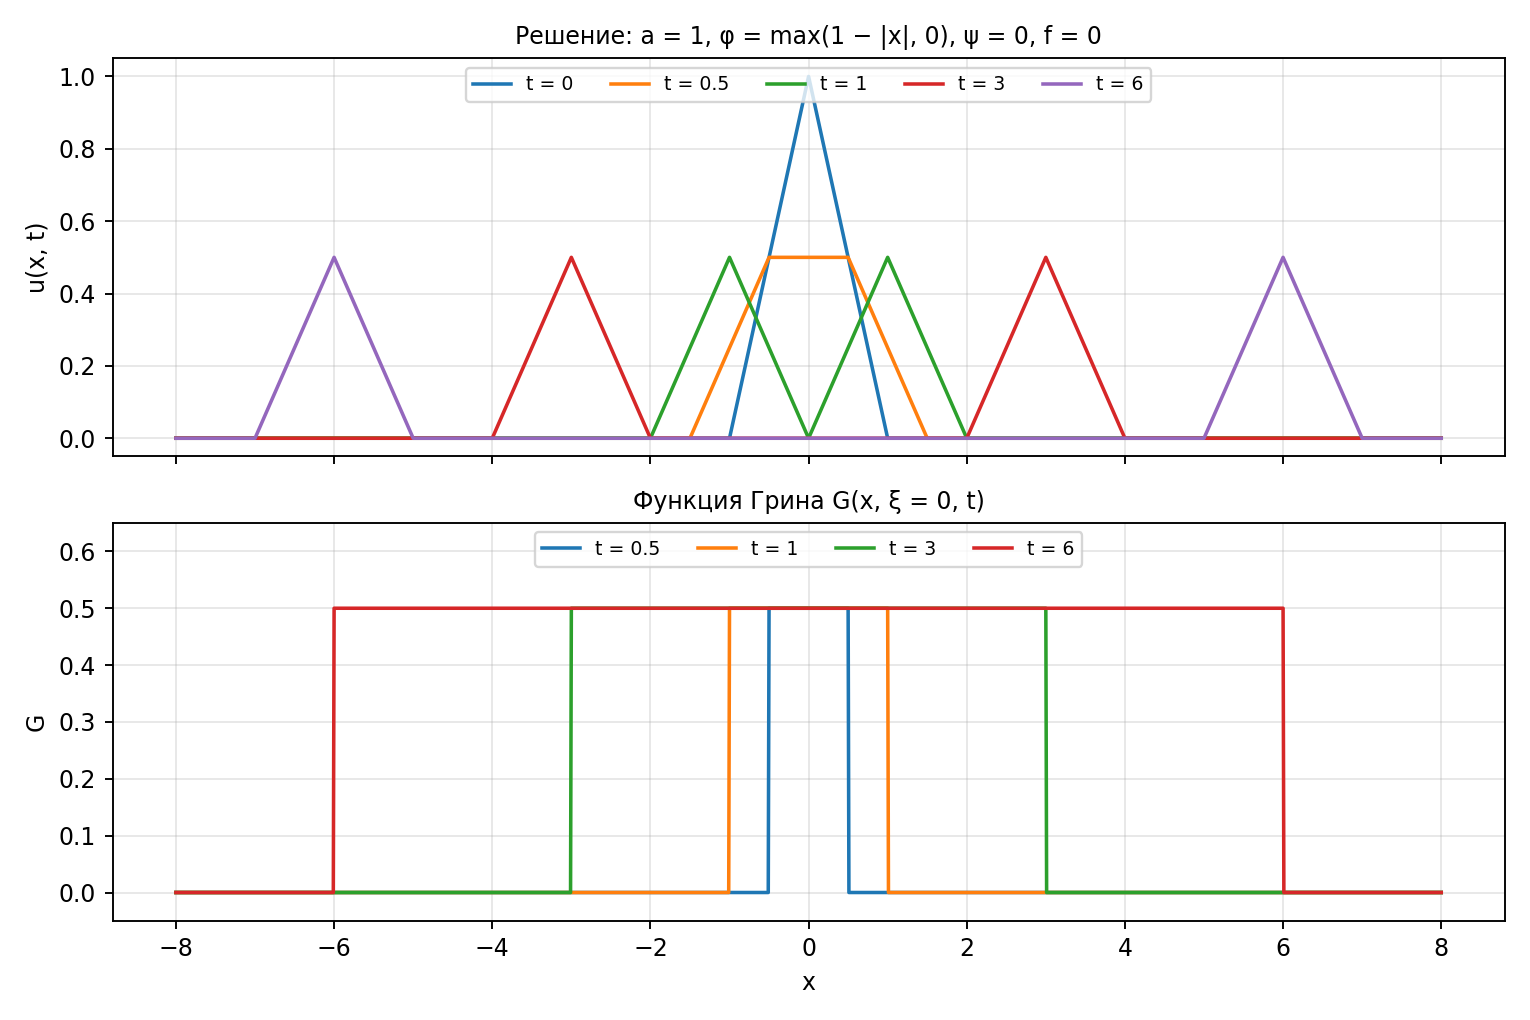
\includegraphics[width=0.88\textwidth]{b_frames.png}
  \caption{Кадры анимации: решение (сверху) и функция Грина (снизу)}
  \label{fig:b-frames}
\end{figure}

На рисунке~\ref{fig:b-terms} показаны вклады второго и третьего слагаемых
формулы~\eqref{eq:uG}: начальный толчок $\psi=e^{-x^2}$ и внешняя сила
$f=e^{-x^2}\sin 3t$.

\begin{figure}[H]
  \centering
  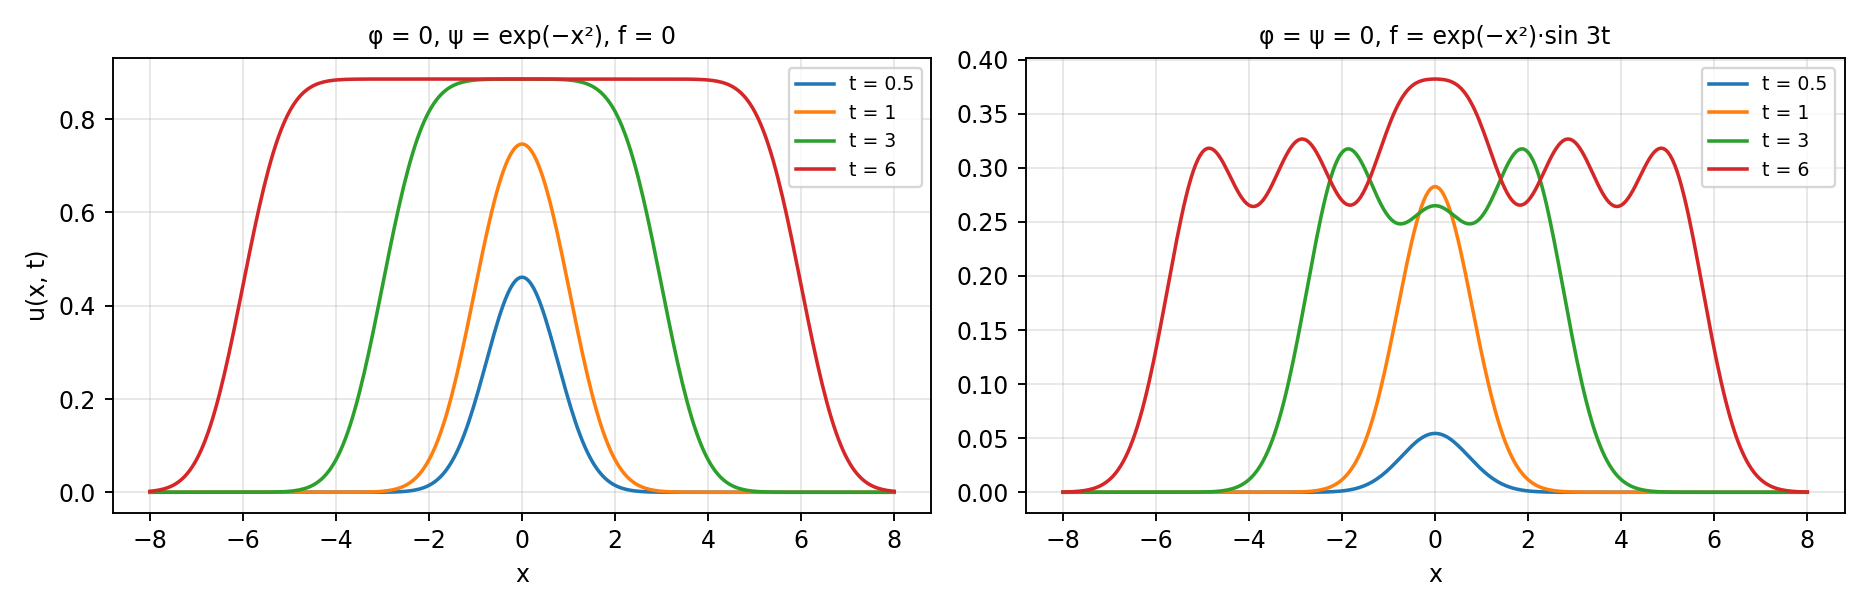
\includegraphics[width=\textwidth]{b_terms.png}
  \caption{Слева~--- только начальная скорость, справа~--- только внешняя сила}
  \label{fig:b-terms}
\end{figure}

\subsection{Проверка}

Результаты сравнения с точными решениями ($a=1{,}5$, $-6\le x\le 6$)
приведены в таблице~\ref{tab:b}.

\begin{table}[H]
  \centering
  \caption{Проверка задания Б}\label{tab:b}
  \begin{tabular}{@{}lll@{}}
    \toprule
    Данные задачи & Точное решение & Отклонение \\
    \midrule
    $\varphi=e^{-x^2}$, $\psi=\sin x$ & формула Даламбера & $<10^{-7}$ \\
    $f=\sin x$ & $\sin x\,(1-\cos at)/a^{2}$ & $<10^{-7}$ \\
    $f=xt$ & $xt^{3}/6$ & $<10^{-9}$ \\
    $\varphi=\max(1-|x|,0)$, $a=1$, $t=10$ & пример лекции 3 & $<10^{-12}$ \\
    \bottomrule
  \end{tabular}
\end{table}

Проверены и свойства функции Грина: $G=0$ при $t\le 0$ и вне конуса
$|x-\xi|\le at$, симметрия $G(x,\xi,t)=G(\xi,x,t)$,
$\int G\,dx=t$. Равенство $\int G_t\varphi\,d\xi=\frac{\partial}{\partial t}\int G\varphi\,d\xi$
подтверждено численным дифференцированием (файл \code{tests/test\_green.py}).

% ======================================================================
\section{Запуск}

\begin{itemize}
  \item \code{python app.py}~--- приложение с интерфейсом (рисунок~\ref{fig:app}):
        вкладки А и Б, поля ввода, ползунок времени, анимация, сохранение PNG и GIF.
  \item \code{python task\_a.py}~--- задание А; без аргументов программа
        спрашивает данные по очереди, клавиша Enter оставляет значение по умолчанию.
  \item \code{python task\_b.py}~--- задание Б, так же.
  \item \code{python -m unittest discover -s tests -t .}~--- 22 теста.
\end{itemize}
Функции вводятся как выражения от \code{x} и \code{t}, например
\code{exp(-(x-5)**2)}, \code{sin(2*t)}, \code{0.3*t}, \code{maximum(1-abs(x),0)}.

\begin{figure}[H]
  \centering
  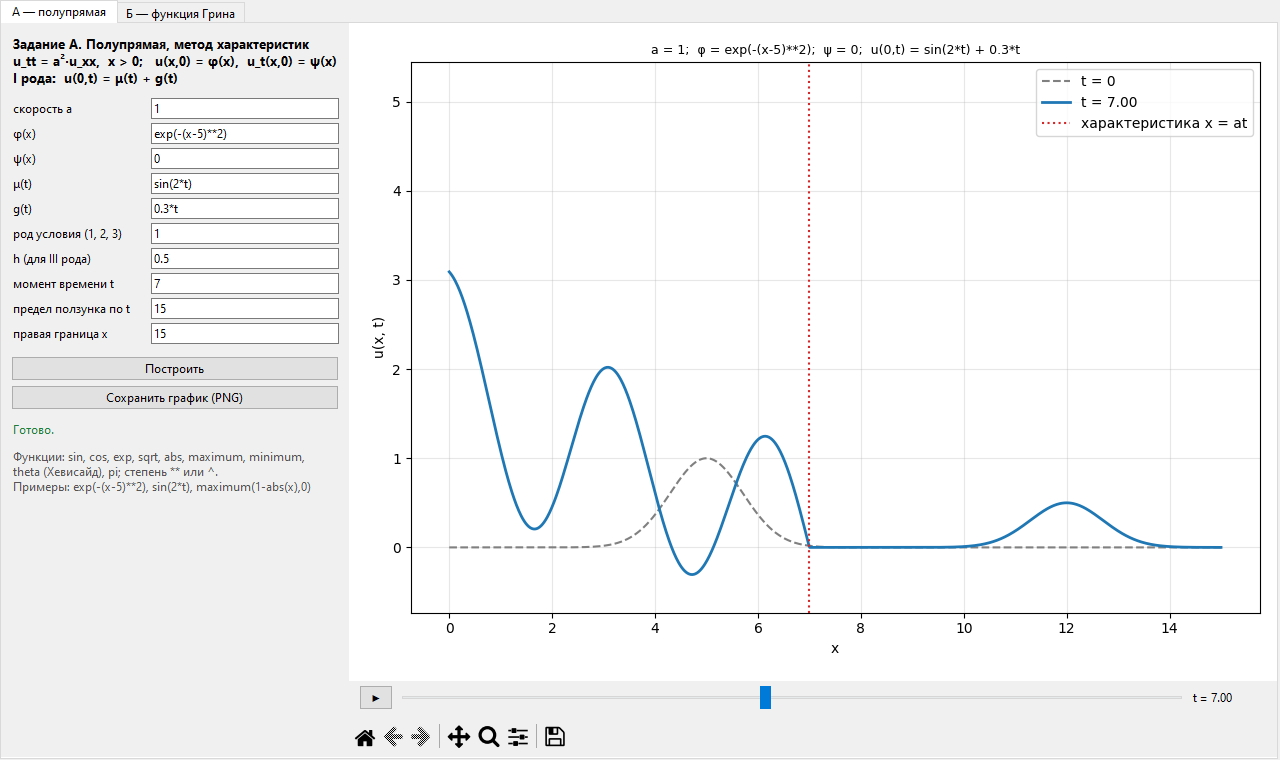
\includegraphics[width=\textwidth]{app_a.png}
  \caption{Окно приложения \code{app.py}, вкладка задания А}
  \label{fig:app}
\end{figure}

\end{document}
